\subsection{Optimal Experimental Design Considerations}

In this section we return to the nonlinear examples presented in the previous chapter and address some choices made in how the experiment was performed.
By revisiting the examples, we demonstrate that the decisions made regarding measurement equipment and/or location have an impact on the reduction of uncertainty and accuracy of the MUD point.
Furthermore, we show that the choices made in the experimental design of previous examples are made for reasons of convenience of exposition.
Changing these assumptions does not alter the viability of the MUD point as an alternative estimator for use parameter identification problems.
We study the impact of more precise measurement devices on the convergence rates for the parameter estimates in Appendix \ref{ext:ode-example} for the problem in \ref{subsec:ode-example} of estimating the rate of exponential decay.
To complement these results, we show them alongside ones generated with equipment that measures at twice the temporal frequency.

In Section~\ref{sec:pde-oed-example}, we also highlight how an awareness of another geometric property of QoI maps---relating to their sensitivity with respect to $\param$---can help improve the accuracy of the MUD estimate.
By placing sensors in locations which exhibit greater sensitivity to the parameter for which the SIP is solved, experimenters can achieve a considerable improvement in the precision of estimating $\paramref$ with an equal number of measurements collected.
A similar complementary problem is solved where information about the sensitivity of measurement locations is used to inform improved placement of a hundred sensors.
In this example, we walk through the sorts of analyses a modeler might conduct in order to select an experimental design through simulation and show a significant improvement in the accuracy of the MUD point.


%%%%%%%%%%%%%%%%%%%%%%%%%%%%%%%%%%%%%%%%%%%%%%%%%%%%%%%%%%%%%%%%%%%%
%%%%%%%%%%%%%%%%%%%%%%%%%%%%%%%%%%%%%%%%%%%%%%%%%%%%%%%%%%%%%%%%%%%%
\FloatBarrier
%%%%%%%%%%%%%%%%%%%%%%%%%%%%%%%%%%%%%%%%%%%%%%%%%%%%%%%%%%%%%%%%%%%%
%%%%%%%%%%%%%%%%%%%%%%%%%%%%%%%%%%%%%%%%%%%%%%%%%%%%%%%%%%%%%%%%%%%%
\subsection{Elliptic PDE Example}\label{sec:pde-oed-example}
We make a slight modification to the Poisson problem from \ref{subsec:pde-example} to make it into a one-dimensional parameter identification problem.
This choice is primarily motivated by the goal of using visual aids to demonstrate slopes corresponding to different measurement locations.
We briefly summarize the experimental set-up again for the reader's convenience.
Consider the following Poisson problem defined on a unit domain $\Omega$:
\begin{equation}\label{eq:pde-equation}
\begin{cases}
\hfill -\nabla \cdot \nabla u &= f \quad\text{on } \Omega \\
\hfill u &= 0 \quad\text{ on } \Gamma_T \cup \Gamma_B \\
\hfill \frac{\partial u}{\partial \mathbf{n}} &= g(x,\param) \quad\text{ on } \Gamma_L \\
\hfill \frac{\partial u}{\partial \mathbf{n}} &= 0 \quad\text{ on } \Gamma_R
\end{cases}
\end{equation}
where $(x_1, x_2) \in \Omega = (0,1)^2$, $\Gamma_T$ is the top, $\Gamma_B$ is the bottom, $\Gamma_L$ and $\Gamma_R$ left and right, respectively.
$\frac{\partial u}{\partial \mathbf{n}}$ denotes the outward normal direction.
We select $g=\param \sin(\pi x_2)$, and show the response surface for $\param = 3$ in the left of Figure~\ref{fig:pde-response}, with darker colors representing more negative values.
The initial density is chosen to be uniform over the interval $\Lambda = (1,5)$, and $f$ is chosen to be $10\exp\{-\frac{(x_1-0.5)^2 + (x_2 - 0.5)^2}{0.02}\}$.


We demonstrate the impact of incorporating more measurements on the ability to estimate $\paramref$.
%This poses a problem for this particular experimental design since it will heavily rely on the way in which the sensor grid is indexed.
%One could place a regular grid of sensors in the interior of $\Omega$ to simulate a structured sensor array.
%However, observe that the response surface shown on the left panel of Figure~\ref{fig:pde-response} exhibit vertical symmetry about the line $x_2=0.5$ (as a result of our choice of $g$).
%For example, if the first half of indexed sensors corresponded to the bottom half of $\Omega$, the incorporation of the second half will be equivalent to having repeated observations.
%To avoid these problems, we instead simulate the sensors as being placed randomly (drawn from uniform distributions), in the interior so that index-dependence becomes irrelevant and probability theory ensures the lack of truly redundant measurement locations.
In \cite{Walsh}, the geometric quantity known as \emph{scaling} inherent to QoI maps is studied with respect to its impact on the precision of solutions to SIPs.
This property corresponds to the average local linear response of the QoI map with respect to changes in $\param$.
In short, if a QoI map (such as one induced by a single measurement), exhibits larger slopes on average over $\pspace$, then it has greater scaling and by implication, more predictive precision.
We demonstrate how an awareness of the QoI's scaling can inform the construction of a more optimal QoI map by way of better selecting the locations of measurement devices.
Here, the assessment of a map's average scaling is identified heuristically through visual inspection of slopes.
Such a graphical comparison of QoI maps can be done without prior knowledge of the scaling property and is not outside the scope of analysis that could be performed during initial investigation into an inverse problem.

%%%%%%%%%%%%%%%%%%%%%%%%%%%%%%%%%%%%%%%%%%%%%%%%%%%%%%%%%%%%%%%%%%%%
\FloatBarrier
%%%%%%%%%%%%%%%%%%%%%%%%%%%%%%%%%%%%%%%%%%%%%%%%%%%%%%%%%%%%%%%%%%%%
\subsubsection{Uninformed Sensor Placement}
First we show that using the sensor-placement strategy introduced in \ref{subsec:pde-example} results in many locations that provide little information to reduce uncertainty in the parameter space.
We consider a selection of $S=1000$ measurement locations in the interior of the response surface chosen by sampling a uniform density over the set $(0.05, 0.95)^2 \subset \Omega$.
We show only the first $100$ measurement locations in plots for visual clarity.
In the rightmost histogram of Figure~\ref{fig:pde-response}, we plot the data generated by each simulated sensor location, and note that many values are near zero as a result of being near boundaries or the right-side of $\Omega$.

\begin{figure}
\centering
  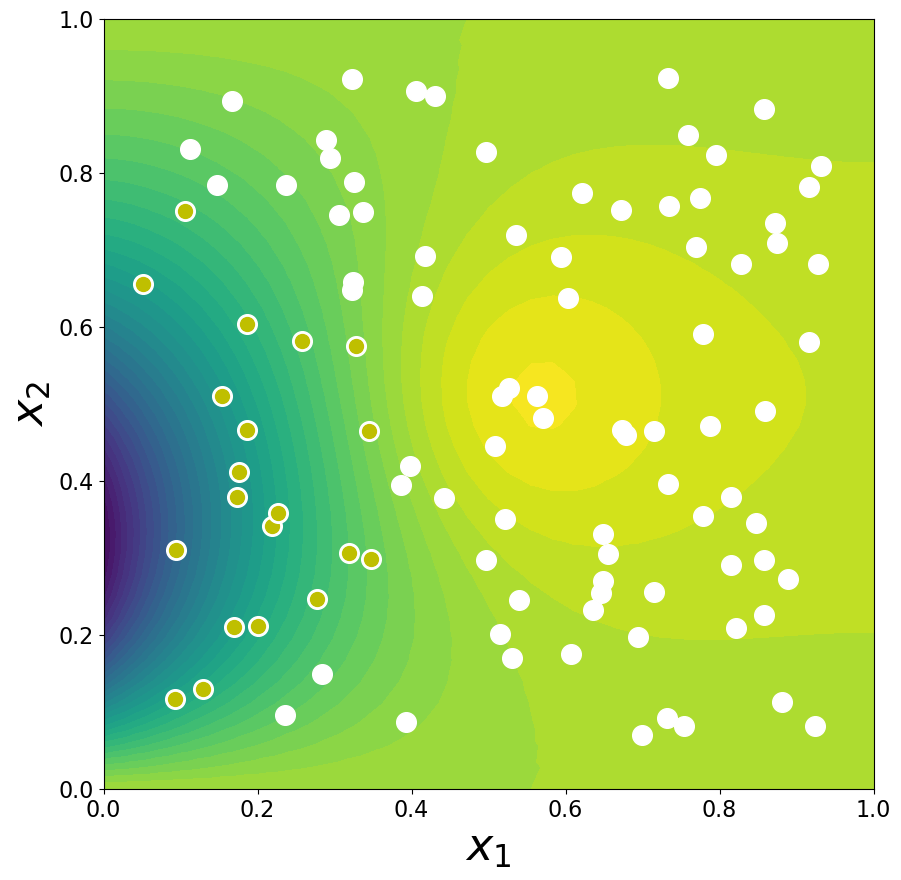
\includegraphics[width=0.25\linewidth]{figures/pde/pde_reference_solution}
  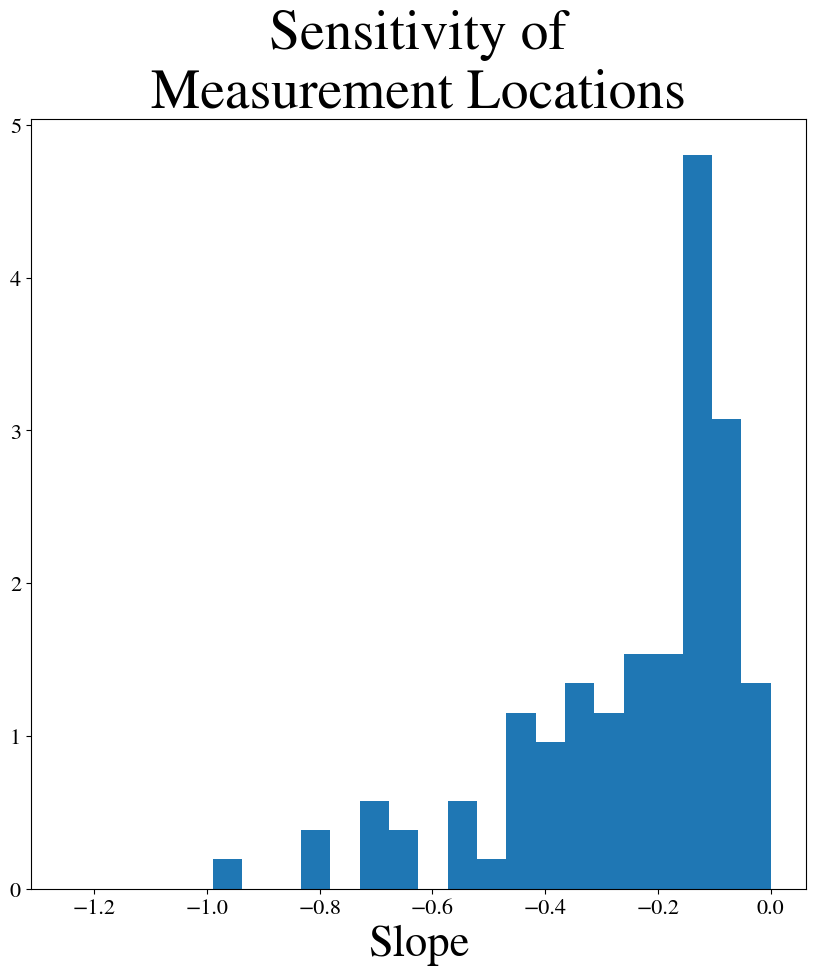
\includegraphics[width=0.25\linewidth]{figures/pde/pde_sensitivity_qoi}
  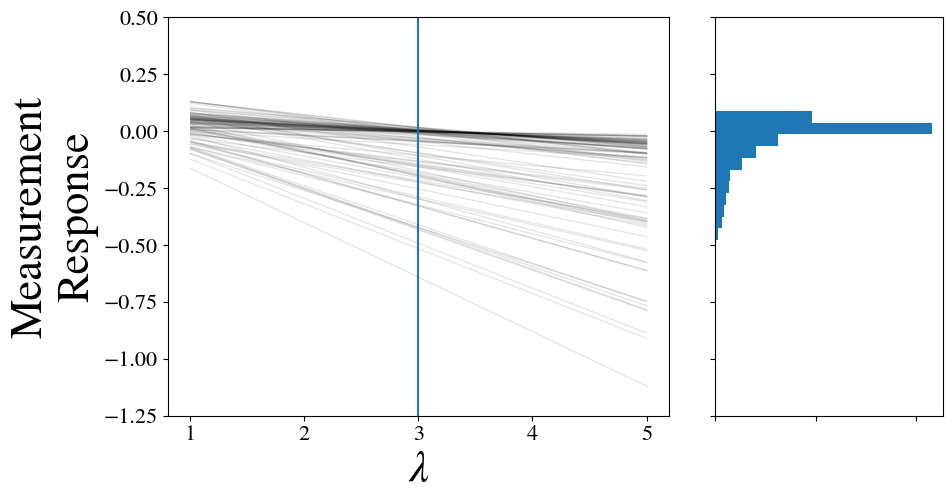
\includegraphics[width=0.45\linewidth]{figures/pde/pde_qoi_response}
\caption{(Left): The function response surface for $u$ solving \eqref{eq:pde-equation} with $S=100$ measurement locations highlighted in white.
The twenty most sensitive location markers are filled.
(Right): The derivative $\partial M_i / \partial \param$ is computed for the $100$ measurement locations and the distribution of the resulting collection of slopes is plotted.
(Center): The values of the response surface at the measurements is shown. The true parameter value $\paramref$ is highlighted with a vertical line, and the values of the response surface conditioned on $\paramref$ are used to form the histogram plotted vertically on the right. Many measurements are near zero.
}
\label{fig:pde-response}
\end{figure}

The measurement response as a function of $\param$ is plotted next to it in the center of \ref{fig:pde-response}, and suggests that the sensors each exhibit linear responses to changes in the parameter.
This observation can be used to visually identify that some measurements are more sensitive than others since the lines from certain sensors have steeper slopes than the majority of locations.
The majority of measurements exhibit almost no sensitivity to changes in $\param$, visually represented by the density of nearly horizontal lines (slopes of zero).
However, some of the sensors have steep slopes, which suggests higher sensitivity to changes in $\param$.
To quantify the variability in the slopes across different sensor locations, we use the smallest and largest samples values of $(\param, u(\param))$ to make a global linear estimate of each one's slope.
We plot the distribution associated with the collection of these slopes in the center histogram of \ref{fig:pde-response}.
%%%%%%%%%%%%%%%%%%%%%%%%%%%%%%%%%%%%%%%%%%%%%%%%%%%%%%%%%%%%%%%%%%%%
% \vfill
\FloatBarrier
%%%%%%%%%%%%%%%%%%%%%%%%%%%%%%%%%%%%%%%%%%%%%%%%%%%%%%%%%%%%%%%%%%%%
\subsubsection{Informed Sensor Placement}
Instead of placing sensors throughout the square interior of $\Omega$ given by $(0.05, 0.95)^2$, we consider how the convergence results would compare if the subdomain for sensors was better selected.
In the left panel of Figure~\ref{fig:pde-response}, the most sensitive measurements are highlighted and appear near the left boundary.
Furthermore, the response surface exhibits horizontal symmetry, so we restrict locations to the bottom half of $\Omega$.
These two observations can inform a new bounding box for consideration of where measurements should be taken.
We perform the same experiment for sensors placed in $(0.05, 0.25)\times(0.05, 0.5)$ (measurement locations drawn from a uniform distribution over this region), and refer to this as the \emph{alternative} experimental design.
The first $100$ of the $1000$ sensor locations sampled is shown in the left panel of \ref{fig:pde-alt-response} and we remark that the most sensitive ones (highlighted) cluster near the center of the left boundary, where the response surface is most negative.


\begin{figure}
\centering
  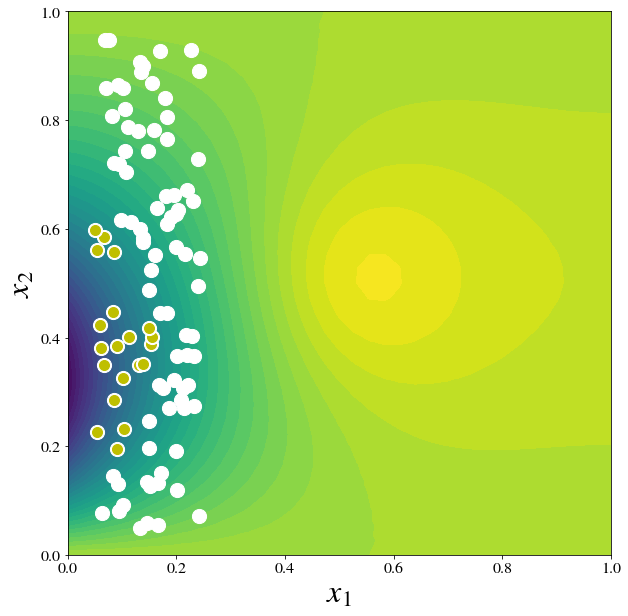
\includegraphics[width=0.25\linewidth]{figures/pde/pde-alt_reference_solution}
  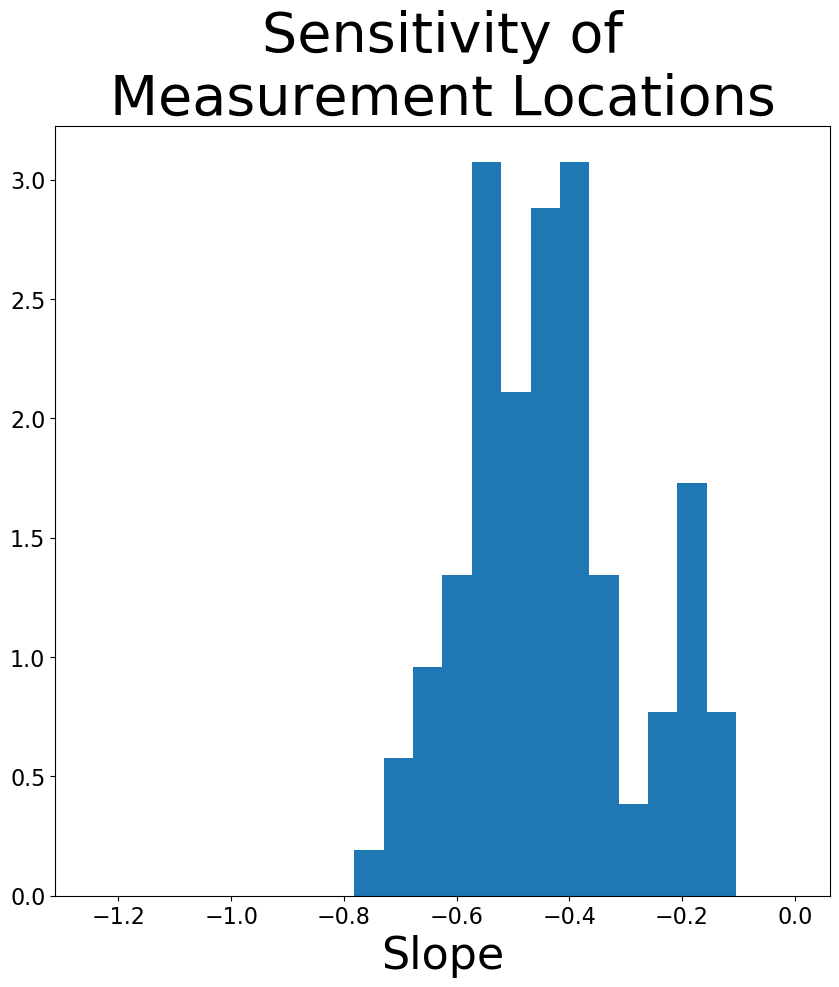
\includegraphics[width=0.25\linewidth]{figures/pde/pde-alt_sensitivity_qoi}
  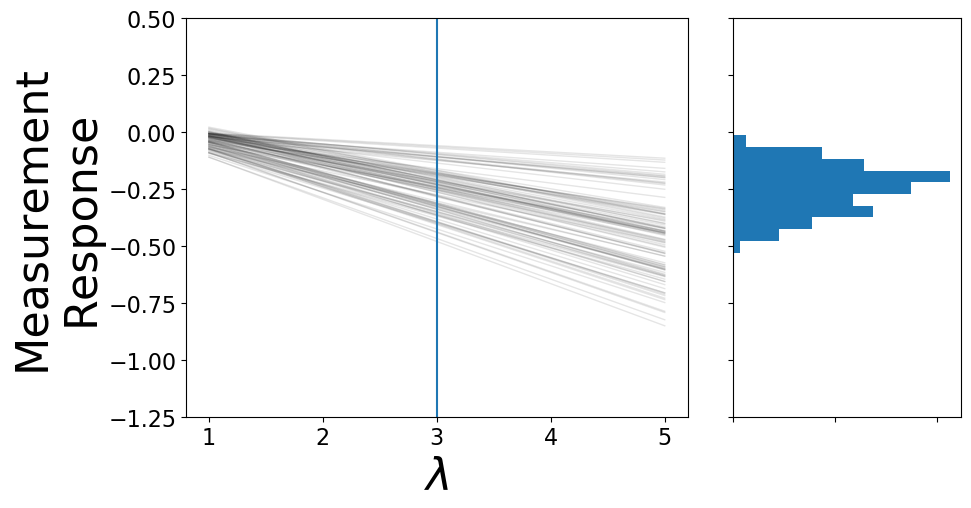
\includegraphics[width=0.45\linewidth]{figures/pde/pde-alt_qoi_response}
  \caption{The same panels as in Figure~\ref{fig:pde-response} but for the placement of sensors informed by the observations about sensitivity incorporated into the experimental design.
  The alternative placement eliminates redundancy induced by the symmetry of the response surface, and is concentrated in the regions which exhibit more sensitivity to changes in $\param$.
  As a result of these choices, we observe less measurements near zero (bottom histogram), and slopes with larger magnitude (top).
  }
\label{fig:pde-alt-response}
\end{figure}

For this alternative design, we show the sensitivity of sensors in the center of \ref{fig:pde-alt-response} and note that there are fewer sensors which exhibit low sensitivity to changes in $\paramref$ in contrast to \ref{fig:pde-response}.
The slopes are again shown in the center of the figure and exhibit a bimodal distribution with a larger portion of the measurements having slopes with magnitude 4-6 times greater than the mode in the center of \ref{fig:pde-response}.
There are also less measurements which take values near zero as well, shown in the rightmost panel of the figures.
The original design exhibited a strong decay in its distribution of measurement values, while the alternative design results in a much more symmetric distribution.

% \vfill
%%%%%%%%%%%%%%%%%%%%%%%%%%%%%%%%%%%%%%%%%%%%%%%%%%%%%%%%%%%%%%%%%%%%
\FloatBarrier
%%%%%%%%%%%%%%%%%%%%%%%%%%%%%%%%%%%%%%%%%%%%%%%%%%%%%%%%%%%%%%%%%%%%
\subsubsection{Comparison of SIP Solutions with Different QoI Maps}

We are interested in knowing how the uncertainty around the parameter estimate (the MUD point) changes as we incorporate more (noisy) data.
To generate convergence plots, we solve the problem repeatedly for $S = 5, 10, 15, 20, 25, 50, 100, 250, 500, \text{ and } 1000$ and take the mean and variance of the twenty trials for each value of $S$.
Consider the convergence plots in Figure~\ref{fig:pde-convergence-obs}, which demonstrates the impact of increasing $S$ on our ability to resolve $\paramref$.

\begin{figure}
  \centering
  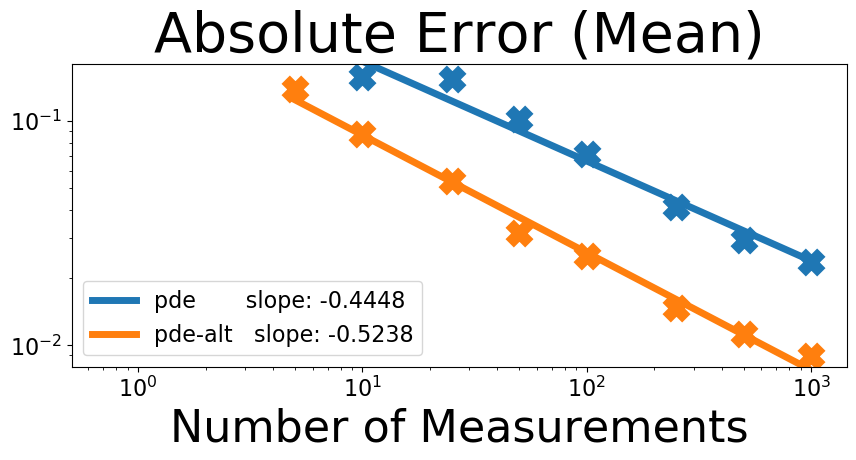
\includegraphics[width=0.475\linewidth]{figures/pde/pde_convergence_mud_obs_mean}
  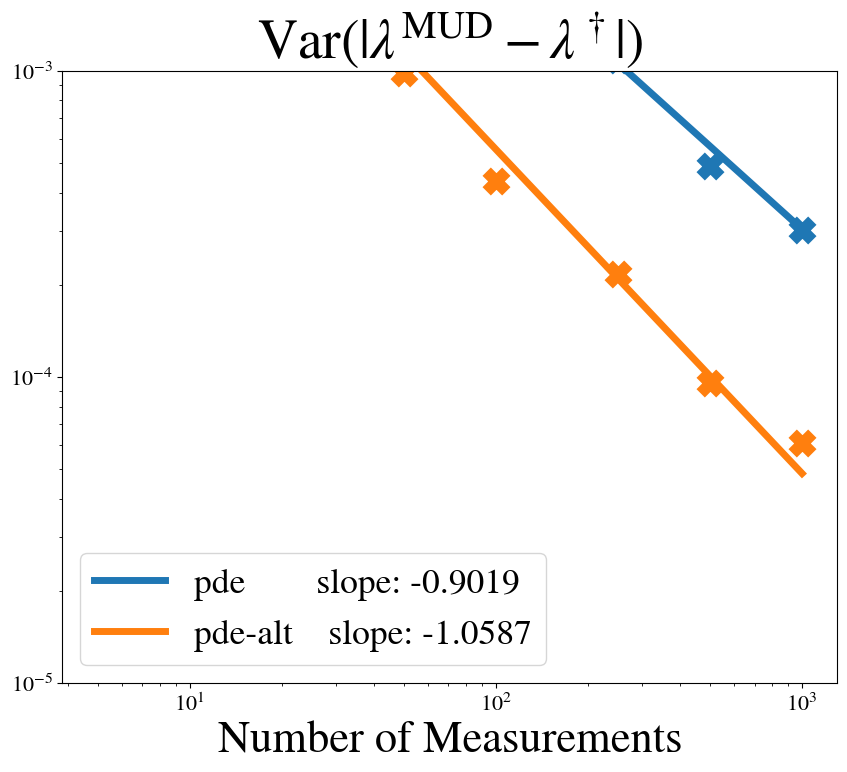
\includegraphics[width=0.475\linewidth]{figures/pde/pde_convergence_mud_obs_var}
  \caption{Convergence of the MUD point (given $N=1E3$ model evaluations) for increasing numbers of observations for randomly placed sensors.
  We observe similar rates of convergence for both arrangements of measurement locations, with a marked improvement in both accuracy and precision when an informed placement is used.
  }
  \label{fig:pde-convergence-obs}
\end{figure}

We show the mean absolute error in the left half of Figure~\ref{fig:pde-convergence-obs} and remark that two decimal places of accuracy can be achieved with approximately $250$ samples instead of the $1000$ required in the left-half.
In Appendix~\ref{ext:pde-tolerance}, we show these results for an experiment conducted with equipment of varying precision.

The convergence results for the original experimental design demonstrate that even randomly placed sensors in the interior of $\Omega$ are suitable for parameter estimation.
However, when we considered sensors that are placed with knowledge about the physical system being studied, more information is learned from the measurement equipment by placing sensors in different locations.
Using the alternative experimental design, we see a reduction of uncertainty in both Figures~\ref{fig:pde-convergence-obs} and \ref{fig:pde-convergence-std}, represented by the persistent vertical displacement between the regression lines for convergence.


%%%%%%%%%%%%%%%%%%%%%%%%%%%%%%%%%%%%%%%%%%%%%%%%%%%%%%%%%%%%%%%%%%%%
%%%%%%%%%%%%%%%%%%%%%%%%%%%%%%%%%%%%%%%%%%%%%%%%%%%%%%%%%%%%%%%%%%%%
\FloatBarrier
%%%%%%%%%%%%%%%%%%%%%%%%%%%%%%%%%%%%%%%%%%%%%%%%%%%%%%%%%%%%%%%%%%%%
%%%%%%%%%%%%%%%%%%%%%%%%%%%%%%%%%%%%%%%%%%%%%%%%%%%%%%%%%%%%%%%%%%%%
%
% \subsection{Concluding Remarks}
% These examples demonstrate that Data--Consistent Inversion can be used for parameter identification as a viable alternative to existing methods.
% Incorporating available observations as we have done in the previous example leaves the output space scalar-valued.
% As the number of parameters grows, this output dimension resulting from such an approach effectively stays fixed.
% These situations are particularly when the DCI approach becomes advantageous over other methods, as it is less sensitive to mistakes in modeling assumptions than other methods for solving inverse problems as we saw with the linear examples in \ref{subsec:linear_examples} \ref{sec:high-dim-linear-example}.
% One can incorporate a much wider variety of prior beliefs about the relative likelihoods of parameters before data is collected without compromising predictive error.
% The DCI approach guarantees that the functional defined (for us, the weighted mean error) will remain accurate in spite of any encoded assumptions that are somehow at odds with data that is subsequently collected.
